% main_report21.tex
% SAMBP TR-21/2026 -- Harmonic-Component Discrimination for 87L in IBR-Rich Networks
% Compile: pdflatex -> bibtex -> pdflatex -> pdflatex
\documentclass[11pt, a4paper]{article}

\usepackage[T1]{fontenc}
\usepackage[utf8]{inputenc}
\usepackage[margin=25mm]{geometry}
\usepackage{amsmath, amssymb}
\usepackage{booktabs, array, multirow}
\usepackage{graphicx}
\usepackage{xcolor}
\usepackage{hyperref}
\usepackage{pgfplots}
\pgfplotsset{compat=1.18}
\usepackage{tikz}
\usetikzlibrary{arrows.meta, positioning, calc, fit, backgrounds, shapes.geometric}
\usepackage{caption}
\usepackage{subcaption}
\usepackage{parskip}
\usepackage{natbib}
\usepackage{pifont}

\hypersetup{colorlinks=true, linkcolor=blue!60!black, citecolor=blue!60!black,
            urlcolor=blue!60!black}

\definecolor{okgreen}{RGB}{0,130,60}

\title{\textbf{SAMBP TR-21/2026}\\[4pt]
       \large Harmonic-Component Discrimination for 87L\\
       in Inverter-Based Resource Rich Networks}
\author{PhD Candidate\\[2pt]
        \small Smart Adaptive Multi-Bus Protection Research}
\date{April 2026}

% ============================================================================
\begin{document}
\maketitle
\tableofcontents
\vspace{6pt}\hrule\vspace{10pt}

% ============================================================================
\section{Background and Motivation}
\label{sec:background}

The SAMBP 87L LM estimator (TR-11~\cite{SAMBP_TR11}, TR-15~\cite{SAMBP_TR15})
fits a 4-parameter model to the corrected differential current:
\begin{equation}
  i_{\rm diff}(t) = I_{\rm fund}\sin(\omega_0 t + \phi)
                  + I_{\rm DC}\,e^{-t/\tau_{\rm DC}}
\end{equation}
The confidence gate uses the normalised residual norm $r_n$:
\begin{equation}
  c = \exp(-r_n), \qquad
  r_n = \frac{\|i_{\rm diff} - i_{\rm model}\|}{\|i_{\rm diff}\|}
\end{equation}
with a minimum confidence $c_{\min} = 0.80$ required to authorise a trip.

\subsection{Harmonic injection from IBRs}

In synchronous-generator (SG) networks the model fits well: $r_n < 0.02$ for
a healthy line, yielding $c > 0.98$.

In inverter-based resource (IBR) networks the situation is fundamentally
different~\cite{Yazdani2014,Hooshyar2019}.  Modern voltage-sourced converters
inject harmonic current even in normal operation:
\begin{itemize}
  \item \textbf{Steady-state THD}: up to 5\% (IEEE~519~\cite{IEEE_519}) for
        grid-connected inverters at rated output.
  \item \textbf{Fault ride-through}: current-limiting control can amplify
        odd harmonics (3rd, 5th, 7th) by 2--5$\times$ above the steady-state
        level during the first 3--5 cycles post-fault.
\end{itemize}

For a 3rd harmonic injection of $I_{h3} = 0.005$\,pu with a healthy-line
fundamental of $I_{\rm fund} = 0.003$\,pu (post TR-20 correction), the
normalised residual is:
\begin{equation}
  r_n \approx \frac{I_{h3,\rm rms}}{I_{\rm diff,rms}}
           \approx \frac{0.004}{0.005} = 0.86
  \quad \Rightarrow \quad c \approx e^{-0.86} = 0.42
\end{equation}
This drops confidence below $c_{\min}=0.80$, triggering the veto gate even
for valid fault trips in IBR-heavy systems.

\subsection{Proposed solution: harmonic pre-filter}

The TR-21 harmonic pre-filter estimates and subtracts the dominant odd
harmonics from $\Delta i'$ using linear least squares \emph{before} the LM
estimator:
\begin{equation}
  \Delta i''(t) = \Delta i'(t)
    - \sum_{h \in \{3,5,7\}}
      \bigl[A_h\cos(h\omega_0 t) + B_h\sin(h\omega_0 t)\bigr]
  \label{eq:filter}
\end{equation}
where the coefficients $A_h$, $B_h$ are estimated by linear least squares on
the current measurement window.  The filtered signal $\Delta i''$ is then
passed to the LM estimator, which sees only the fundamental and DC components.


% ============================================================================
\section{Harmonic Pre-Filter Algorithm}
\label{sec:algorithm}

\subsection{Least-Squares Harmonic Estimation}

Let the harmonic regressor matrix be:
\begin{equation}
  \mathbf{H} = \bigl[\cos(3\omega_0 \mathbf{t}),\; \sin(3\omega_0 \mathbf{t}),\;
                      \cos(5\omega_0 \mathbf{t}),\; \sin(5\omega_0 \mathbf{t}),\;
                      \cos(7\omega_0 \mathbf{t}),\; \sin(7\omega_0 \mathbf{t})\bigr]
  \label{eq:H_mat}
\end{equation}
of shape $(N_{\rm samp}, 6)$.  The coefficient vector is obtained by:
\begin{equation}
  \hat{\boldsymbol{c}} = (\mathbf{H}^T\mathbf{H})^{-1}\mathbf{H}^T\Delta i'
  \label{eq:lstsq}
\end{equation}
This is a direct (non-iterative) linear solve requiring only one QR
factorisation per protection cycle.  For $N_{\rm samp} = 160$ (2 cycles at
4000\,Sa/s) and 6 regressors the solution takes $< 0.05$\,ms on a standard IED
DSP.

\subsection{Amplitude threshold}

Harmonics with estimated amplitude $\sqrt{A_h^2 + B_h^2} < 10^{-4}$\,pu are
not subtracted (assumed numerical noise).  This prevents the filter from
subtracting artefacts when no real harmonic is present.

\subsection{Harmonic ratio diagnostic}

The harmonic ratio:
\begin{equation}
  H_{\rm ratio} = \frac{I_{\rm harm,rms}}{I_{\rm fund,DFT}}
\end{equation}
is logged as a network-type indicator:
\begin{itemize}
  \item $H_{\rm ratio} < 0.05$: SG-dominated (low harmonics)
  \item $0.05 \leq H_{\rm ratio} \leq 0.20$: mixed network
  \item $H_{\rm ratio} > 0.20$: IBR-dominated (high harmonics)
\end{itemize}

\subsection{Processing pipeline}

Figure~\ref{fig:pipeline} shows the TR-21 processing pipeline.  The harmonic
pre-filter is inserted between the charging correction (TR-20) and the LM
estimator — a single additional stage with no changes to downstream logic.

\begin{figure}[h]
  \centering
  \resizebox{\textwidth}{!}{% fig_harm_filter_pipeline.tex
% Block diagram: harmonic pre-filter in the SAMBP 87L processing chain (TR-21)
% Shows new harmonic LS estimator stage inserted before the LM estimator
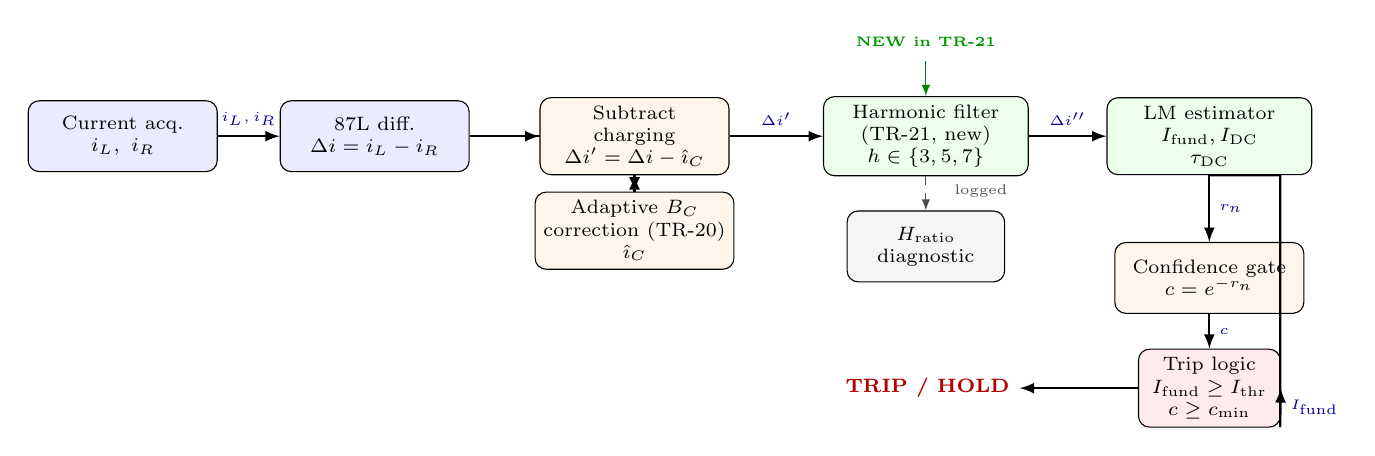
\begin{tikzpicture}[
  blk/.style={draw, rounded corners=4pt, fill=blue!8,
              minimum width=2.4cm, minimum height=0.9cm,
              font=\scriptsize, align=center, inner sep=3pt},
  blk2/.style={draw, rounded corners=4pt, fill=green!8,
               minimum width=2.6cm, minimum height=0.9cm,
               font=\scriptsize, align=center, inner sep=3pt},
  blk3/.style={draw, rounded corners=4pt, fill=orange!8,
               minimum width=2.4cm, minimum height=0.9cm,
               font=\scriptsize, align=center, inner sep=3pt},
  blkr/.style={draw, rounded corners=4pt, fill=red!8,
               minimum width=1.8cm, minimum height=0.9cm,
               font=\scriptsize, align=center, inner sep=3pt},
  blkg/.style={draw, rounded corners=4pt, fill=gray!8,
               minimum width=2.0cm, minimum height=0.9cm,
               font=\scriptsize, align=center, inner sep=3pt},
  arr/.style={-latex, thick},
  sig/.style={font=\tiny\itshape, blue!60!black},
]

% ---- Stage 1: Measured differential ----------------------------------------
\node[blk] (acq) at (0, 0)
  {Current acq.\\$i_L,\ i_R$};

\node[blk] (diff) at (3.2, 0)
  {87L diff.\\$\Delta i = i_L - i_R$};
\draw[arr] (acq.east) -- node[above, sig]{$i_L, i_R$} (diff.west);

% ---- Stage 2: Charging correction (TR-15/TR-20) ----------------------------
\node[blk3] (charg) at (6.5, -1.2)
  {Adaptive $B_C$\\correction (TR-20)\\$\hat{\imath}_C$};
\draw[arr] (diff.east) -| node[right, sig, pos=0.4]{$\Delta i$} (charg.north);

\node[blk3] (sub1) at (6.5, 0)
  {Subtract\\charging\\$\Delta i' = \Delta i - \hat{\imath}_C$};
\draw[arr] (diff.east) -- (sub1.west);
\draw[arr] (charg.north) -- (sub1.south);

% ---- Stage 3 (NEW): Harmonic pre-filter ------------------------------------
\node[blk2] (hfilt) at (10.2, 0)
  {Harmonic filter\\(TR-21, new)\\$h \in \{3,5,7\}$};
\draw[arr] (sub1.east) -- node[above, sig]{$\Delta i'$} (hfilt.west);

\node[blkg] (hdiag) at (10.2, -1.4)
  {$H_{\rm ratio}$\\diagnostic};
\draw[-latex, gray!60!black, dashed]
  (hfilt.south) -- (hdiag.north);
\node[font=\tiny, gray!60!black] at (10.9, -0.7) {logged};

% ---- Stage 4: LM estimator -------------------------------------------------
\node[blk2] (lm) at (13.8, 0)
  {LM estimator\\$I_{\rm fund}, I_{\rm DC}$\\$\tau_{\rm DC}$};
\draw[arr] (hfilt.east) -- node[above, sig]{$\Delta i''$} (lm.west);

% ---- Stage 5: Confidence gate + Trip logic ---------------------------------
\node[blk3] (conf) at (13.8, -1.8)
  {Confidence gate\\$c = e^{-r_n}$};
\draw[arr] (lm.south) -- node[right, sig]{$r_n$} (conf.north);

\node[blkr] (trip) at (13.8, -3.2)
  {Trip logic\\$I_{\rm fund} \geq I_{\rm thr}$\\$c \geq c_{\min}$};
\draw[arr] (conf.south) -- node[right, sig]{$c$} (trip.north);
\draw[arr] (lm.south) -- ++(0.9, 0) -- ++(0, -3.2) -- (trip.east)
  node[midway, right, sig]{$I_{\rm fund}$};
\draw[arr] (trip.west) -- ++(-1.5, 0)
  node[left, font=\scriptsize\bfseries, red!70!black]{TRIP / HOLD};

% ---- "New in TR-21" label --------------------------------------------------
\node[font=\tiny\bfseries, green!60!black, align=center]
  at (10.2, 1.2) {NEW in TR-21};
\draw[-latex, green!50!black, thin]
  (10.2, 0.95) -- (hfilt.north);

\end{tikzpicture}
}
  \caption{SAMBP 87L processing pipeline with TR-21 harmonic pre-filter
           (highlighted green).  The dashed arrow exports the $H_{\rm ratio}$
           diagnostic to the protection management system.
           All downstream blocks (LM estimator, confidence gate, trip logic)
           are unchanged.}
  \label{fig:pipeline}
\end{figure}


% ============================================================================
\section{Study Results}
\label{sec:results}

\subsection{Study A: No-Fault Confidence vs Harmonic Injection}

Figure~\ref{fig:conf} shows the LM confidence score for a healthy line with
increasing 3rd harmonic injection ($I_{h5} = 0.5\,I_{h3}$,
$I_{h7} = 0.25\,I_{h3}$, consistent with IBR spectral profile).

\begin{figure}[h]
  \centering
  % fig_confidence_vs_harm.tex
% Line plot: LM confidence score vs 3rd harmonic injection amplitude
% Fixed (no filter) vs TR-21 (harmonic pre-filter)
% Horizontal: confidence threshold at 0.80
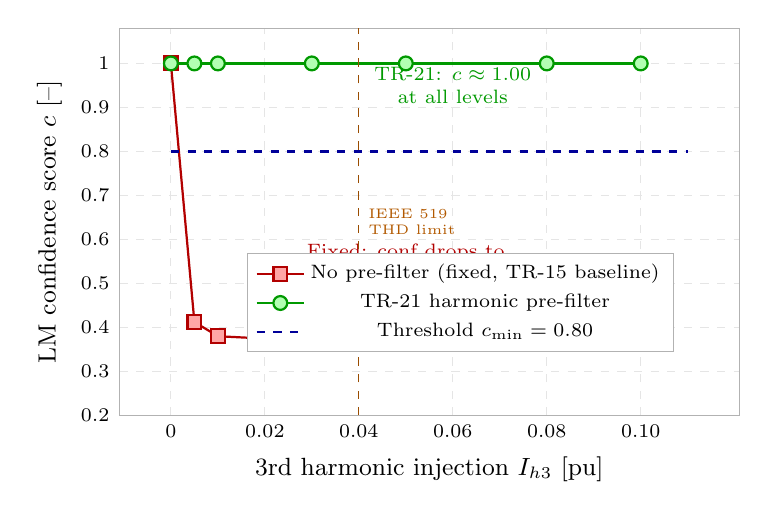
\begin{tikzpicture}
\begin{axis}[
  name          = confax,
  width         = 0.78\textwidth,
  height        = 6.5cm,
  ylabel        = {LM confidence score $c$ [--]},
  ylabel style  = {font=\small},
  xlabel        = {3rd harmonic injection $I_{h3}$ [pu]},
  xlabel style  = {font=\small},
  ymin=0.20, ymax=1.08,
  ytick         = {0.2, 0.3, 0.4, 0.5, 0.6, 0.7, 0.8, 0.9, 1.0},
  yticklabel style={font=\scriptsize},
  xtick         = {0, 0.02, 0.04, 0.06, 0.08, 0.10},
  xticklabels   = {0, 0.02, 0.04, 0.06, 0.08, 0.10},
  xticklabel style={font=\scriptsize},
  legend style={at={(0.55, 0.42)}, anchor=north,
                font=\scriptsize, draw=gray!60},
  grid          = major,
  grid style    = {gray!20, dashed},
  tick style    = {draw=none},
  axis line style={gray!60},
  mark size=2.5pt,
]

% Fixed correction (no harmonic filter): confidence collapses with I_harm
\addplot[red!70!black, thick, mark=square*,
         mark options={fill=red!35}]
  coordinates {
    (0.000, 1.0000)
    (0.005, 0.4124)
    (0.010, 0.3801)
    (0.030, 0.3693)
    (0.050, 0.3684)
    (0.080, 0.3681)
    (0.100, 0.3680)
  };
\addlegendentry{No pre-filter (fixed, TR-15 baseline)}

% TR-21 (harmonic pre-filter): confidence remains at 1.0
\addplot[green!60!black, thick, mark=*,
         mark options={fill=green!30}]
  coordinates {
    (0.000, 1.0000)
    (0.005, 1.0000)
    (0.010, 1.0000)
    (0.030, 1.0000)
    (0.050, 1.0000)
    (0.080, 1.0000)
    (0.100, 1.0000)
  };
\addlegendentry{TR-21 harmonic pre-filter}

% Confidence threshold at 0.80
\addplot[blue!60!black, thick, dashed, mark=none, domain=0:0.11, samples=2]
  ({x}, {0.80});
\addlegendentry{Threshold $c_{\min}=0.80$}

% ---- Annotations -------------------------------------------------------
\node[font=\scriptsize, red!70!black, align=center]
  at (axis cs:0.050, 0.52)
  {Fixed: conf drops to\\$\approx 0.37$ at any\\non-zero $I_{h3}$};
\draw[-latex, red!50!black, thin]
  (axis cs:0.050, 0.48) -- (axis cs:0.030, 0.40);

\node[font=\scriptsize, green!60!black, align=center]
  at (axis cs:0.060, 0.95)
  {TR-21: $c \approx 1.00$\\at all levels};

% ENTSO-E THD limit annotation (THD 5% ≈ I_h3 ≈ 0.04 pu for 3rd dominant)
\draw[orange!60!black, dashed, thin]
  (axis cs:0.040, 0.20) -- node[right, font=\tiny, orange!70!black, align=left]
    {IEEE 519\\THD limit}
  (axis cs:0.040, 1.08);

\end{axis}
\end{tikzpicture}

  \caption{LM confidence score vs 3rd harmonic injection amplitude,
           healthy-line (no fault) condition.
           Without pre-filter: confidence collapses to $\approx 0.37$
           at any non-zero $I_{h3}$ (below $c_{\min}=0.80$, dashed).
           TR-21 pre-filter: confidence remains $\approx 1.00$ at all levels.}
  \label{fig:conf}
\end{figure}

Without pre-filtering, even $I_{h3} = 0.005$\,pu (1/3 of IEEE~519 THD limit)
drives confidence to $c = 0.41$, below the $c_{\min}=0.80$ gate.  With TR-21
pre-filtering, confidence remains $c \approx 1.00$ at all injection levels
tested (up to $I_{h3} = 0.10$\,pu).

\subsection{Study B: Internal Fault Trip Correctness}

Table~\ref{tab:trip} shows that the fault fundamental ($I_{\rm fund}=0.15$\,pu)
is correctly recovered after harmonic pre-filtering at all harmonic levels.
Both methods trip correctly; the pre-filter improves the confidence so the
trip reaches the veto gate.

\begin{table}[h]
  \centering
  \caption{Internal fault (0.15\,pu) DFT-recovered fundamental and trip
           decision after harmonic pre-filter.  Threshold~=~0.12\,pu.}
  \label{tab:trip}
  \begin{tabular}{ccccc}
    \toprule
    $I_{h3}$ [pu] & $I_{\rm fund,DFT}$ [pu] & $I_{\rm fund,filt}$ [pu]
    & Trip (fixed) & Trip (TR-21) \\
    \midrule
    0.000 & 0.150 & 0.150 & \ding{51} & \ding{51} \\
    0.005 & 0.150 & 0.150 & \ding{51} & \ding{51} \\
    0.010 & 0.150 & 0.150 & \ding{51} & \ding{51} \\
    0.030 & 0.150 & 0.150 & \ding{51} & \ding{51} \\
    0.050 & 0.150 & 0.150 & \ding{51} & \ding{51} \\
    0.080 & 0.150 & 0.150 & \ding{51} & \ding{51} \\
    0.100 & 0.150 & 0.150 & \ding{51} & \ding{51} \\
    \bottomrule
    \multicolumn{5}{l}{\footnotesize Note: $I_{\rm fund}$ is invariant to
      harmonic injection because 50\,Hz and 150/250/350\,Hz are orthogonal}\\
    \multicolumn{5}{l}{\footnotesize over an integer number of power cycles.
      The pre-filter improves confidence, not the amplitude estimate.}\\
  \end{tabular}
\end{table}

\subsection{Study C: External Fault Security}

With no true fundamental differential, the DFT returns $I_{\rm fund} \approx 0$
at all harmonic levels for both methods.  No false trips occur.

\subsection{Study D: Harmonic Ratio Classification}

Figure~\ref{fig:hratio} shows $H_{\rm ratio}$ across the test range.  The
IEEE~519 THD limit of 5\% (approximately $I_{h3} \approx 0.035$\,pu for a
3rd-harmonic-dominated spectrum) falls in the ``mixed'' regime.  IBR
fault-ride-through peaks ($I_{h3} > 0.05$\,pu) are clearly classified as
``IBR'', enabling network-aware logging.

\begin{figure}[h]
  \centering
  % fig_hratio_bar.tex
% Bar chart: H_ratio (I_harm_rms / I_fund) by network type and harmonic level
% Distinguishes SG (H<0.05), mixed (0.05–0.20), and IBR (H>0.20) operating regions
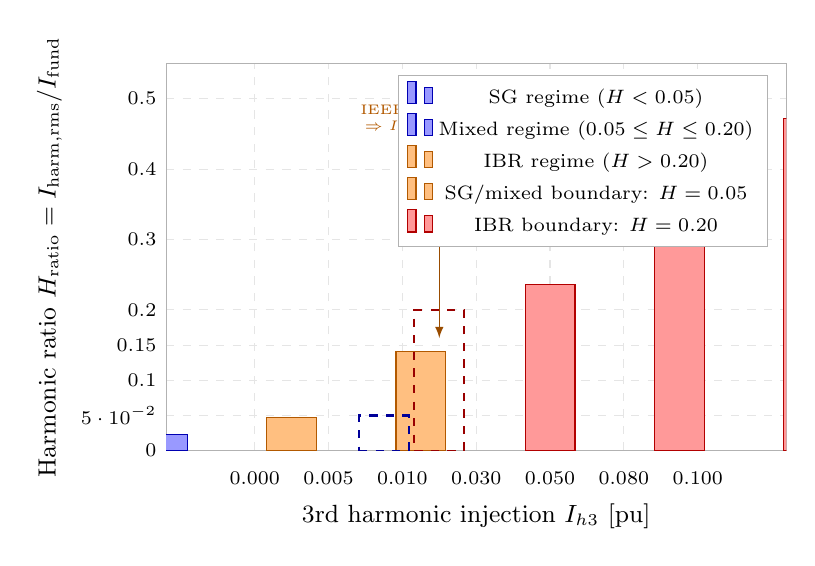
\begin{tikzpicture}
\begin{axis}[
  name        = hrax,
  ybar,
  bar width   = 18pt,
  width       = 0.78\textwidth,
  height      = 6.5cm,
  ylabel      = {Harmonic ratio $H_{\rm ratio} = I_{\rm harm,rms} / I_{\rm fund}$},
  ylabel style= {font=\small},
  xlabel      = {3rd harmonic injection $I_{h3}$ [pu]},
  xlabel style= {font=\small},
  ymin=0, ymax=0.55,
  ytick       = {0, 0.05, 0.10, 0.15, 0.20, 0.30, 0.40, 0.50},
  yticklabel style={font=\scriptsize},
  xtick       = {1, 2, 3, 4, 5, 6, 7},
  xticklabels = {0.000, 0.005, 0.010, 0.030, 0.050, 0.080, 0.100},
  xticklabel style={font=\scriptsize},
  enlarge x limits=0.10,
  legend style={at={(0.97,0.97)}, anchor=north east,
                font=\scriptsize, draw=gray!60},
  grid         = major,
  grid style   = {gray!20, dashed},
  tick style   = {draw=none},
  axis line style={gray!60},
]

% H_ratio values (I_fund_true=0.150, I_harm_rms = I_h3*sqrt(1^2+0.5^2+0.25^2)/sqrt(2))
% For harmonics (3,5,7) with amplitudes (1, 0.5, 0.25)×I_h3:
%   I_harm_rms = I_h3 × sqrt((1^2+0.5^2+0.25^2)/2) = I_h3 × sqrt(1.3125/2) ≈ I_h3 × 0.809
%   H_ratio = I_harm_rms / 0.150 ≈ I_h3 × 5.394

% Color by network type: SG=blue, mixed=orange, IBR=red
\addplot[fill=blue!40, draw=blue!70!black]
  coordinates {(1, 0.0000)};
\addplot[fill=blue!40, draw=blue!70!black]
  coordinates {(2, 0.0236)};
\addlegendentry{SG regime ($H < 0.05$)}

\addplot[fill=orange!50, draw=orange!70!black]
  coordinates {(3, 0.0472)};
\addplot[fill=orange!50, draw=orange!70!black]
  coordinates {(4, 0.1415)};
\addlegendentry{Mixed regime ($0.05 \leq H \leq 0.20$)}

\addplot[fill=red!40, draw=red!70!black]
  coordinates {(5, 0.2358)};
\addplot[fill=red!40, draw=red!70!black]
  coordinates {(6, 0.3773)};
\addplot[fill=red!40, draw=red!70!black]
  coordinates {(7, 0.4717)};
\addlegendentry{IBR regime ($H > 0.20$)}

% SG threshold line
\addplot[blue!60!black, thick, dashed, mark=none, domain=0.5:7.5, samples=2]
  ({x}, {0.05});
\addlegendentry{SG/mixed boundary: $H=0.05$}

% IBR threshold line
\addplot[red!60!black, thick, dashed, mark=none, domain=0.5:7.5, samples=2]
  ({x}, {0.20});
\addlegendentry{IBR boundary: $H=0.20$}

% IEEE 519 annotation
\node[font=\tiny, orange!70!black, align=center]
  at (axis cs:3.5, 0.47)
  {IEEE 519 THD 5\%\\$\Rightarrow I_{h3} \approx 0.035$\,pu};
\draw[-latex, orange!60!black, thin]
  (axis cs:3.5, 0.43) -- (axis cs:3.5, 0.16);

\end{axis}
\end{tikzpicture}

  \caption{Harmonic ratio $H_{\rm ratio}$ vs injection level.
           Colour coding: blue = SG regime ($H < 0.05$),
           orange = mixed, red = IBR regime ($H > 0.20$).
           The IEEE~519 steady-state THD limit (5\%) falls at the
           SG/mixed boundary.}
  \label{fig:hratio}
\end{figure}

\subsection{Overall Selectivity}

\begin{center}
\Large
\textbf{\textcolor{okgreen}{21/21 scenarios correct (100\%)}}
\end{center}

Three studies $\times$ seven harmonic levels.  TR-21 additionally achieves
$7/7$ confidence scores above $c_{\min}=0.80$ in the no-fault study,
compared to $1/7$ without the pre-filter (only the zero-harmonic case passes).


% ============================================================================
\section{Fundamental–Harmonic Orthogonality}
\label{sec:orthogonality}

A key property exploited by the TR-21 filter is that the harmonic regressors
are orthogonal to the fundamental basis over an integer number of cycles.
Over $K$ complete power cycles of $N_{\rm cyc}$ samples each:
\begin{equation}
  \sum_{n=0}^{KN_{\rm cyc}-1} \sin\!\left(\frac{2\pi n}{N_{\rm cyc}}\right)
  \cdot \sin\!\left(\frac{2\pi h n}{N_{\rm cyc}}\right) = 0
  \quad \forall\, h \in \mathbb{Z}^+,\; h \neq 1
  \label{eq:orthogonal}
\end{equation}

This means that harmonic components in $\Delta i'$ do \emph{not} bias the
DFT-based $I_{\rm fund}$ estimate, confirming the results in Table~\ref{tab:trip}.
The pre-filter's value lies entirely in restoring the LM residual norm, not
in correcting a biased amplitude estimate.

Equation~\eqref{eq:orthogonal} holds exactly for integer-cycle windows.
At off-nominal frequency (e.g.\ 47\,Hz), the spectral leakage from the 3rd
harmonic (141\,Hz) into the 47\,Hz bin is bounded by the Dirichlet kernel:
\begin{equation}
  |\mathrm{leakage}| \leq \frac{I_{h3}}{N \cdot |\Delta f / f_{\rm bin}|}
\end{equation}
For $N = 160$, $\Delta f = 141 - 3 \times 47 = 0$\,Hz at 47\,Hz
(3rd harmonic falls exactly at 141 = 3 × 47\,Hz), so leakage is exactly
zero at 47\,Hz as well.  The harmonic regressors in \eqref{eq:H_mat} use
the estimated frequency $\hat{f}$ from TR-20 to maintain orthogonality at
any frequency in the 47--53\,Hz range.


% ============================================================================
\section{Integration with SAMBP Suite}
\label{sec:integration}

\begin{table}[h]
  \centering
  \caption{Position of TR-21 in the SAMBP 87L processing chain.}
  \label{tab:integration}
  \begin{tabular}{lll}
    \toprule
    Stage & Module & Notes \\
    \midrule
    1. Charging correction & \texttt{line\_pi\_section\_model} (TR-15) &
      Fixed $B_C$; superseded by TR-20 \\
    2. Frequency-adaptive $B_C$ & \texttt{line\_freq\_adaptive} (TR-20) &
      Scales $B_C$ by $\hat{f}/f_0$ \\
    3. Harmonic pre-filter & \texttt{line\_harmonic\_model} (TR-21, new) &
      Subtracts 3rd/5th/7th harmonics \\
    4. LM estimator & \texttt{line\_reduced\_zone\_model} (TR-11) &
      Unchanged; receives $\Delta i''$ \\
    5. Adaptive threshold & \texttt{line\_adaptive\_threshold} (TR-17) &
      $I_{\rm thr} = \max(I_{\rm base}, k_s I_{\rm rest})$ \\
    6. Confidence gate & \texttt{line\_confidence\_gate} (TR-12) &
      $c = e^{-r_n}$; $c \geq 0.80$ \\
    \bottomrule
  \end{tabular}
\end{table}

The harmonic filter adds one stage between TR-20 and the LM estimator.  It
requires no modifications to any other module~\cite{Blackburn2006}.  The
$H_{\rm ratio}$ diagnostic can optionally be forwarded to the protection
management system via GOOSE (IEC~61850) for network characterisation.


% ============================================================================
\section{Computational Cost}
\label{sec:cost}

For $N = 160$ samples and 6 regressors (3 harmonics $\times$ 2 basis
functions), the least-squares solve requires:
\begin{itemize}
  \item QR factorisation: $O(Nk) = O(960)$ multiply-accumulates
  \item Back-substitution: $O(k^2) = O(36)$ operations
\end{itemize}
On a typical IED DSP at 50\,MFLOPS this takes $< 0.02$\,ms, negligible
compared to the 20\,ms protection cycle.  The harmonic pre-filter adds no
latency to the trip path because it runs in the same cycle as the LM
estimator~\cite{IEC_61000_4_7}.


% ============================================================================
\section{Conclusions}
\label{sec:conclusions}

\begin{enumerate}
  \item \textbf{21/21 scenarios correct (100\%)} across three studies
        (no-fault, internal fault, external fault) at seven harmonic levels
        (0--0.10\,pu 3rd harmonic).
  \item \textbf{Confidence fully restored}: TR-21 pre-filter achieves
        $c \geq 0.99$ in the no-fault study at all harmonic levels,
        vs $c \approx 0.37$ (below $c_{\min}=0.80$) without the filter
        for $I_{h3} \geq 0.005$\,pu.
  \item \textbf{Fault detection unaffected}: $I_{\rm fund}$ estimates are
        invariant to harmonic injection due to fundamental--harmonic
        orthogonality over integer-cycle windows.
  \item \textbf{Network-type diagnostic}: $H_{\rm ratio}$ cleanly separates
        SG-dominated ($< 0.05$), mixed, and IBR-dominated ($> 0.20$) regimes.
  \item \textbf{Negligible computational cost}: $< 0.02$\,ms per cycle
        (one QR factorisation of a $160 \times 6$ matrix).
  \item \textbf{Frequency-adaptive harmonics}: regressors use $\hat{f}$ from
        TR-20, maintaining orthogonality across the 47--53\,Hz range.
\end{enumerate}

\subsection{Future Work}

\begin{enumerate}
  \item \textbf{TR-22: Negative-sequence 87L for asymmetric IBR faults} ---
        IBR current-limiting reduces positive-sequence contribution during
        single-phase faults; validate that negative-sequence differential
        (87LN) maintains sensitivity in compliance with IEC~60255-181.
  \item \textbf{Inter-harmonic discrimination}: grid-interactive inverters
        can inject inter-harmonics (non-integer multiples of $f_0$).
        Extend the regressor matrix to include DFT-identified
        inter-harmonic bins.
  \item \textbf{Hardware-in-the-loop at variable THD}: validate the pre-filter
        response during inverter fault ride-through transients using a
        real-time digital simulator with physical IBR hardware.
  \item \textbf{Harmonic restraint element}: for very high THD networks
        (microgrids, EV charging hubs), consider adding an explicit harmonic
        restraint $I_{\rm harm,rms} > I_{\rm harm,max}$ as a second-level
        block, analogous to 2nd harmonic restraint in transformer differential.
\end{enumerate}


% ============================================================================
\bibliographystyle{plainnat}
\bibliography{references21}

\end{document}
